\documentclass[UTF8]{article}
\usepackage{bm}
\usepackage{amsmath}
\usepackage{cases}
\usepackage{cite}
\usepackage{graphicx}
\usepackage[margin=1in]{geometry}
\geometry{a4paper}
\usepackage{fancyhdr}
\pagestyle{fancy}
\usepackage{wrapfig}
\fancyhf{}
\usepackage{float}  %设置图片浮动位置的宏包
\usepackage{subfigure}
\usepackage{caption}
\usepackage{booktabs}
\usepackage{listings}
\usepackage{xcolor}
\usepackage{multirow}
\lstset{numbers=left, %设置行号位置
	numberstyle=\tiny, %设置行号大小
	keywordstyle=\color{blue}, %设置关键字颜色
	commentstyle=\color[cmyk]{1,0,1,0}, %设置注释颜色
	frame=single, %设置边框格式
	escapeinside=``, %逃逸字符(1左面的键),用于显示中文
	breaklines, %自动折行
	extendedchars=false, %解决代码跨页时,章节标题,页眉等汉字不显示的问题
	xleftmargin=2em,xrightmargin=2em, aboveskip=1em, %设置边距
	tabsize=4, %设置tab空格数
	showspaces=false %不显示空格
}

\title{Measurement of the focal length of thin lenses}
\author{by 22 Artificial Intelligence ChenxuZhang}
\date{2023.4.19}
\pagenumbering{arabic}

\begin{document}
	
	\fancyhead[L]{ChenxuZhang}
	\fancyhead[R]{ID 202264691028}
	\fancyfoot[C]{\thepage}
	
	\maketitle
	\tableofcontents
	\newpage
	
	\section{Abstract}
A thin lens is one in which the central thickness of the lens is negligible compared to the radius of curvature of the sphere. Currently, thin lenses are used in a wide range of imaging They are used in a wide range of applications, such as astronomy, medicine, digital cameras, mobile phones, etc. Depending on the application and purpose for which the thin lens is used The measurement of the focal length of a thin lens is essential as different lenses or sets of lenses should be selected for different applications and purposes.

There are many methods of measuring the focal length of thin lenses, such as the geometric, Fourier and instrumental methods. Geometric methods include, self-collimation The geometric method includes the self-collimation method, the object-image distance method, the primary imaging method and the twice-imaging method; the instrumental method includes the resistance wire method and the spectrophotometer method. In this experiment we In this experiment, we use the self-collimation method, the primary imaging method and the secondary imaging method (conjugate method) to measure the focal length of a convex lens, and the object distance and image distance methods to measure the focal length of a concave lens. The focal length of a concave lens is measured using the self-collimation method.\\
	
	\textbf{Result:}We calculated the focal lengths of the final convex lens No. 2 and No. 3, as well as the concave lens No. 4, as follows:$f_2 = 19.47\pm 0.04cm \quad f_3 = 25.76  \pm 0.04cm \quad f_4 = 5.85\pm 0.19cm$\\
	\textbf{Key Words: Thin lenses, Focal length, Primary imaging method, Secondary imaging method, Parallel light measurement,Object distance and image distance measurement}
	
	
	\section{Purpose of the experiment}
   $\bm{A}$.Learn about the co-axial adjustment of simple optical systems.\\
   $\bm{B}$.Learn several ways to measure the focal length of convex and concave lenses.\\
   $\bm{C}$.Experiment with ways to measure the focal length of thin lenses and deepen your understanding of the principles of optical imaging.\\
   $\bm{D}$.Understand the principles of optical imaging and the thin lens formula.
      

	\section{Experimental apparatus}
	
		\subsection{Optical Instruments Group}
		The optical instrument set consists of the following items: optical tool holders, convex lenses, concave lenses, parallel white light sources, sodium lamps, object screens, pincushion screens, flat reflectors, etc.
			\begin{figure}[H]
					\centering
					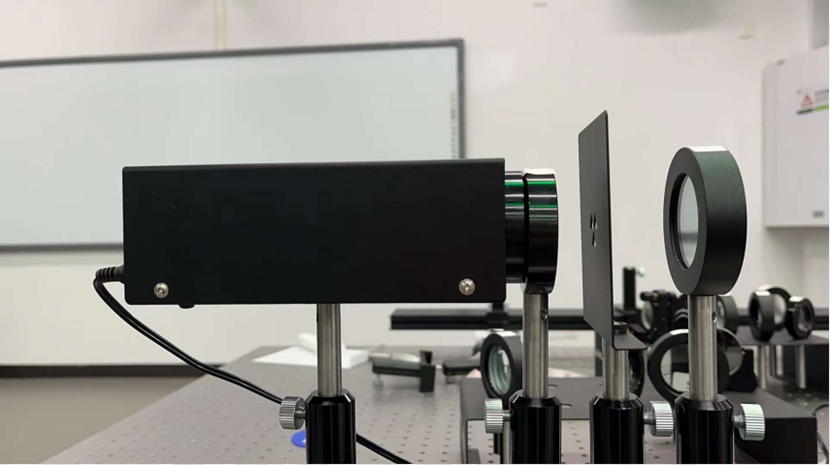
\includegraphics[clip,scale=0.9,trim={0 50 0 30}]{fig/fig1.png}
					\caption{Parallel white light source}
					\label{figure.1}
				\end{figure}
		\begin{itemize}
		\item Optical Bench - An apparatus used to perform experiments in optics, consisting of a long, flat board with various components mounted on it, such as lenses, mirrors, and light sources.
		\item Convex Lens - A lens that bulges outward in the middle and converges light rays to a point, also known as a converging lens.
		\item Concave Lens - A lens that curves inward in the middle and diverges light rays, also known as a diverging lens.
		\item Parallel White Light Source - A source of light that emits rays of light that are parallel to each other.
		\item Sodium Lamp - A type of electric lamp that produces yellow light by ionizing sodium vapor.
		\item Object Screen - A surface on which an image is projected or formed, often used in optical experiments.
		\item Crosswire Screen - A screen with two thin wires or threads that cross each other at right angles, used for measuring the position and size of images.
		\item Flat Mirror - A reflective surface that is flat and smooth, used to reflect light in a predictable way.
		\end{itemize}
		
		\begin{figure}[H]
			\begin{minipage}[t]{0.65\linewidth}
				\centering
				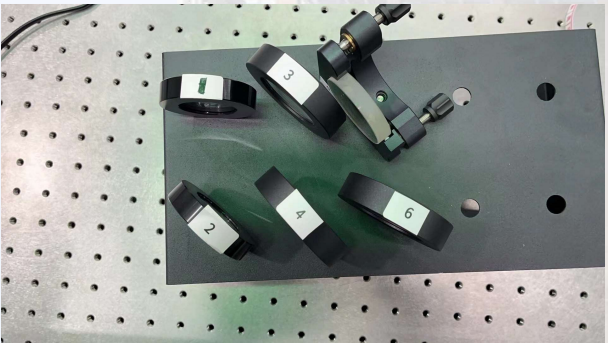
\includegraphics[clip,scale=0.75,trim={0 0 0 0}]{fig/fig2.png}
				\caption{Convex and Concave Lenses}
				\label{figure.2}
			\end{minipage}
			\begin{minipage}[t]{0.35\linewidth}
				\centering
				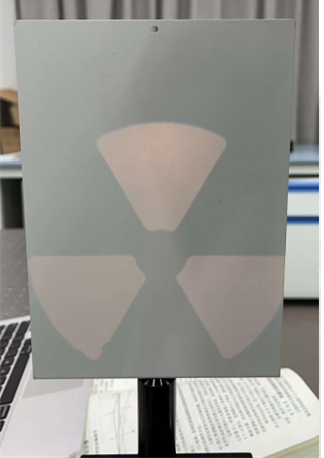
\includegraphics[clip,scale=0.55]{fig/fig3.png}
				\caption{Object screen showing the shape of the Pinnacle screen}
				\label{figure.3}
			\end{minipage}
		\end{figure}
	    
	 

	    \subsection{Other equipment and assembly of equipment}
	    Other equipment includes metre rulers, goggles etc. Meters are mainly used to measure the distance between optical instruments, while goggles are used to protect the measurer's eyes from glare when measuring degrees. At the same time, the environment of the experiment is also very important: in order to be able to observe the imaging better, we try to place the experimental site in low light to minimise the interference of ambient light with the experiment.
	   \begin{figure}[H]
	   					\centering
	   					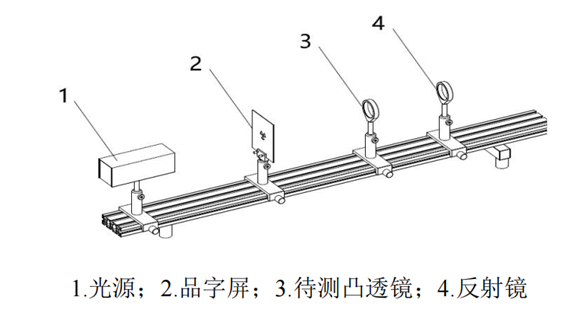
\includegraphics[clip,scale=1,trim={0 30 0 0}]{fig/fig4.png}
	   					\caption{Diagram of optical instrument placement}
	   					\label{figure.4}
	   \end{figure}
	   				
       During the experiment we need to position the experimental optical equipment correctly. We need to place the equipment on the slides of the base in the appropriate order, which may not always be the same for each experiment. Afterwards, adjust the height of the optical instruments to ensure that they are on the same level and contour.
       
      
	\section{Experimental principles}
    Lenses can be divided into two main categories: convex lenses (also known as positive lenses or converging lenses), which act as a converging lens for light. The other type concave lenses (also known as negative or diverging lenses), which diffuse the light.
    
    Under near-optical conditions (light close to the optical axis and at a small angle to the optical axis), the equation for imaging thin lenses (Gauss's formula) is
    \begin{eqnarray}
    \frac{1}{\upsilon } +\frac{1}{u}  =  \frac{1}{f}  
    \end{eqnarray}
    
    Where u is the object distance, v is the image distance and f is the focal length. Its positive and negative values are: u and v are positive for real objects and real images; u is positive and v is negative for imaginary objects and imaginary images; f is positive for convex lenses and negative for concave lenses.
   
    
	\subsection{Measurement of the focal length of a convex lens}
	\subsubsection{Parallel light source focusing method for rapid measurement of convex lens focal lengths}
     The distance from the white screen to the lens is the focal length of the lens f. This is one of the easiest and fastest ways to measure the focal length of a convex lens. This is the easiest and quickest way to measure the focal length of a convex lens, but in many cases the laboratory is not equipped with a parallel light source and we have to use other methods to measure it.
     \begin{figure}[H]
     	   					\centering
     	   					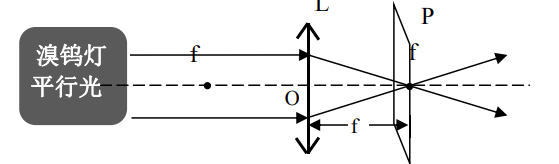
\includegraphics[clip,scale=1,trim={0 0 0 0}]{fig/fig5.png}
     	   					\caption{Diagram of optical instrument placement}
     	   					\label{figure.5}
     	   \end{figure}
     The measurement here uses the property that a convex lens will converge parallel rays of light at the focal length, making it easy to measure but subject to some error.
     
     \subsubsection{Measuring the focal length of a convex lens by primary imaging}
     As shown in Fig.6, on the precision guide, place in turn the illuminator, the object screen (pintle screen or mono screen or mono needle), the convex lens to be measured and the image screen, and set to co-axial. Adjust the position of the convex lens or the object or image screen back and forth along the guide rail until a clear image is obtained on the image screen. until a clear object image is obtained on the image screen, note down the coordinates of the position of the object screen, convex lens and image screen, and obtain the object and image distances. Calculate the focal length f by taking it into the equation.
      \begin{figure}[H]
      			\begin{minipage}[t]{0.5\linewidth}
      				\centering
      				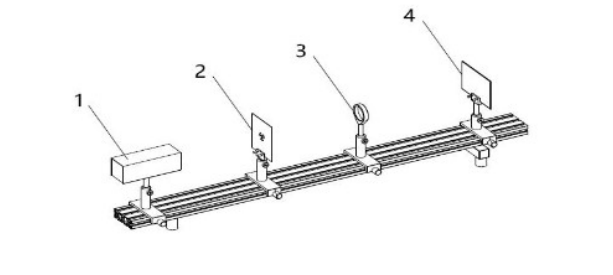
\includegraphics[clip,scale=0.75,trim={0 0 0 0}]{fig/fig6.png}
      				\caption{Primary imaging method}
      				\label{figure.6}
      			\end{minipage}
      			\begin{minipage}[t]{0.5\linewidth}
      				\centering
      				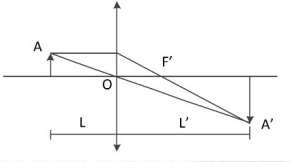
\includegraphics[clip,scale=1.2]{fig/fig7.png}
      				\caption{Object screen showing the shape of the Pinnacle screen}
      				\label{figure.7}
      			\end{minipage}
      		\end{figure}
	The details are as follows:
	\begin{itemize}
	\item Place an object (a luminous object) that serves as a light source between one and two times the focal length of a convex lens.
	\item The light emitted by the object passes through the convex lens and forms an enlarged image on the other side of the lens at a distance twice the focal length away.
	\item The focal length of the lens is denoted by $F'$. The object, denoted by $A$, is located at a distance $L$ from the lens, and its real image, denoted by $A'$, is formed on the other side of the lens at a distance $L'$.
	\item This setup satisfies the equation $\frac{1}{\upsilon } +\frac{1}{u}  =  \frac{1}{f}$, or equivalently, $\frac{1}{L} +\frac{1}{L'}  =  \frac{1}{F'}$. By measuring the object distance and image distance, the focal length can be determined.
	\end{itemize}
	
	\subsubsection{Secondary imaging method (conjugate method)}
	Arrange the optical path according to Fig.8. Select different values of D for D > 4f, move the lens L so that the image screen appears as a clear magnified image and a reduced image respectively, record the coordinates of the object screen, the image screen and the positions of the magnified and reduced images, obtain the values of D and d and substitute them into equation  to calculate the focal length f.
	\begin{figure}[H]
	     	\centering
	     	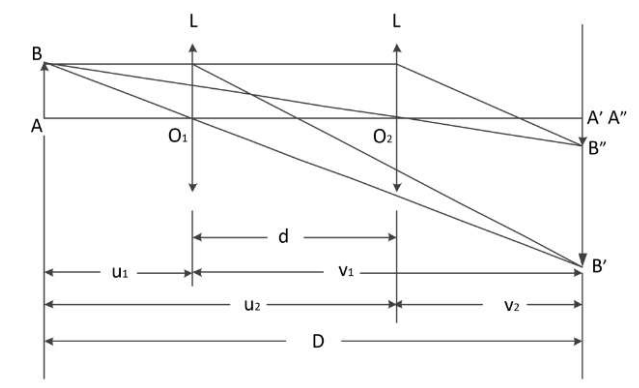
\includegraphics[clip,scale=1,trim={0 0 0 0}]{fig/fig8.png}
	     	\caption{Secondary imaging method for measuring the focal length of a convex lens}
	     	\label{figure.8}
	\end{figure}
	The formula is derived as follows:
	\begin{eqnarray}
	\begin{cases}
	 \frac{1}{u_1}+\frac{1}{D-u_1}  =  \frac{1}{f}   \\
	\frac{1}{u_{1}+d}+\frac{1}{D-u_{1}-d}  =  \frac{1}{f}   
	\end{cases}
	\qquad \Rightarrow \qquad u_1  = \frac{D-d}{2} 
	\end{eqnarray}
	
	Taking the above equation into the formula one can go on to derive the expression for $f$:
	\begin{eqnarray}
	f  =  \frac{D^2-d^2}{4D}  =  \frac{(D+d)(D-d)}{4D}  
	\end{eqnarray}
	
    From the above equation, the focal length f of the convex lens under test can be found when the distance D between the object and image screens and the displacement d during the two imaging sessions of the lens L are measured.
    
	\subsection{Determination of the focal length of a concave lens}
    Because a concave lens is a diverging lens, a real object passing through a concave lens does not produce a real image on the screen, so its focal length always has to be measured A convex lens is used to create a virtual object for the concave lens, which in turn creates a real image from the concave lens.
    
    Object and image distance method for measuring the focal length of a concave lens:
    
    A convex lens is used to make the object $A$ a reduced real image $A'$ on the image screen. Insert a concave lens $L2$ between the convex lens $L1$ and the image screen and treat the image formed by the convex lens as an object (virtual object) of $L2$ with a negative object distance $u$. Move the image screen appropriately to obtain a real image of the virtual object $A"$ with a positive image distance $v$. The focal length of the concave lens can be found by substituting the object and phase distances into the formula $f$.
    
    	\begin{figure}[H]
    	     	\centering
    	     	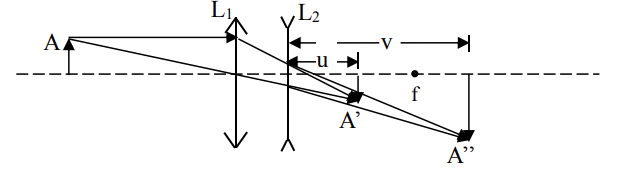
\includegraphics[clip,scale=1,trim={0 0 0 0}]{fig/fig9.png}
    	     	\caption{Object and image distance method for measuring the focal length of a concave lens}
    	     	\label{figure.9}
    	\end{figure}
    
    In addition, according to the reversibility of the optical path, it can be seen from Fig. 9 that the object $A"$ can be taken as an orthogonal reduced virtual image $A'$ through the concave lens $L2$, then $v$ is the object distance (positive) and $u$ is the image distance (negative) in the diagram.
    
    \begin{eqnarray}
    \frac{1}{f}  = \frac{1}{u}-\frac{1}{\upsilon }   
    \end{eqnarray}
    
    This method requires attention to the position of the concave lens, which should be as shown in Fig. 9, to satisfy $u < f$. If $u > f$, the image will not be a real image $A''$, but a magnified orthostatic virtual image.
    
    The details are as follows:
    \begin{itemize}
    \item Because a concave lens is a diverging lens, an object passing through it cannot form a real image on a screen. Therefore, when measuring its focal length, a convex lens is always used to create a virtual object for the concave lens to form a real image from. The blue lens is convex and the orange lens is concave.
    \item Using the convex lens to create a reduced real image $A'$ on the screen, insert the concave lens $L2$ between the convex lens $L1$ and the screen, and treat the image formed by the convex lens as the object for $L2$ (a virtual object). The object distance $u$ is negative, and by adjusting the position of the screen, the real image $A"$ of the virtual object can be obtained with an image distance of $f$.
    \end{itemize}
    

	\section{Contents and Steps}
	\subsection{Co-axial adjustment of optical elements}
	In order to make the light a near-axis light, the optics must first be adjusted to be co-axial. The requirements for adjusting the co-axiality of the optical elements on the optical tool holders are The optical axis of each lens coincides, the central part of the object is on the optical axis, the object surface, the image surface is perpendicular to the optical axis, the optical axis is parallel to the optical tool holder guide rail. The co-axial adjustment should be carried out in two steps:
	\subsubsection{Rough Tuning}
	The light source, object and lens are placed close together in the light fixture holder and carefully observed by eye, adjusting the height and left and right of each optical element so that the centre of the light source, object and lens are roughly in a straight line parallel to the light fixture holder. Make the centre of the light source, the centre of the object and the centre of the lens roughly in a straight line parallel to the light holder.
	
	\subsubsection{Fine tuning}
	Fine tuning follows the imaging laws of the lens to determine if the optics are co-axial. The following is an example of the adjustment method using a single lens.
	\begin{itemize}
	\item Adjust the image to have uniform brightness and completeness. Pull the object screen and the image screen apart on the guide rail to a distance greater than 4f, and move the converging lens between them to form clear magnified and reduced images on the image screen. The formed image must be complete and have uniform brightness. If not, adjust the light source or the object screen accordingly.
    \item Adjust the vertical alignment of the image center. Move lens L to produce a clear magnified image on the image screen, and mark the center position as O'. Then move lens L to produce a clear reduced image on the image screen, and mark the center position as O". If the two centers are not aligned vertically, move lens L towards the object screen to produce a clear magnified image on the image screen, and adjust the height of the object screen to align O' and O". Then move lens L towards the image screen to produce a clear reduced image on the image screen, and check if O' and O" coincide. This adjustment technique in optical experiments is usually called "chasing the large image with the small image".
    \end{itemize}
    
    \begin{figure}[H]
        	     	\centering
        	     	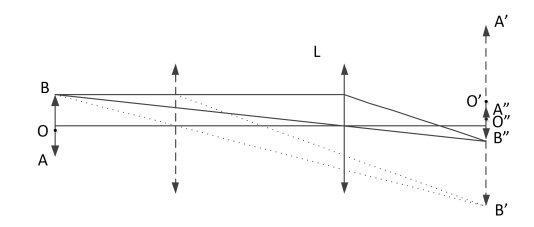
\includegraphics[clip,scale=1,trim={0 0 0 0}]{fig/fig10.png}
        	     	\caption{Co-axial adjustment}
        	     	\label{figure.10}
     \end{figure}
    
    When adjusting, note that if the O' point is above the O" point, then the object centre O is below the adjustment optical axis and the O point should be moved up to bring the O point down closer to the O" point; conversely the O point should be brought down.
    
    Adjust the two image centres to coincide laterally. Adjust the transverse screw adjustment handwheel on the slider of each optical element on the guide.
    
    \subsection{Measuring the focal length of a convex lens}
    \begin{itemize}
    \item Measuring the focal length of convex lens 1 and convex lens 2 by focusing with a parallel light source: \\
    The distance between the white screen and the focal length of the convex lens is the focal length of the convex lens. The distance between the white screen and the convex lens is the focal length of the convex lens f. The measurement is repeated three times for each lens.
    \end{itemize}
    
    \begin{figure}[H]
          			\begin{minipage}[t]{0.5\linewidth}
          				\centering
          				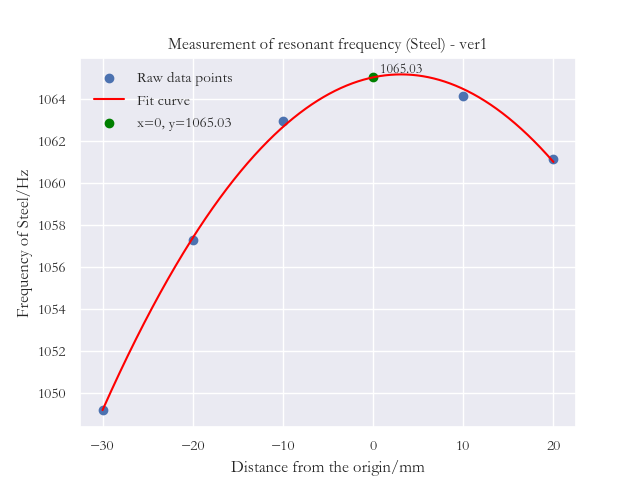
\includegraphics[clip,scale=0.05,trim={0 400 0 400}]{fig/fig11.jpg}
          				\caption{Lens measurement No. 2}
          				\label{figure.11}
          			\end{minipage}
          			\begin{minipage}[t]{0.5\linewidth}
          				\centering
          				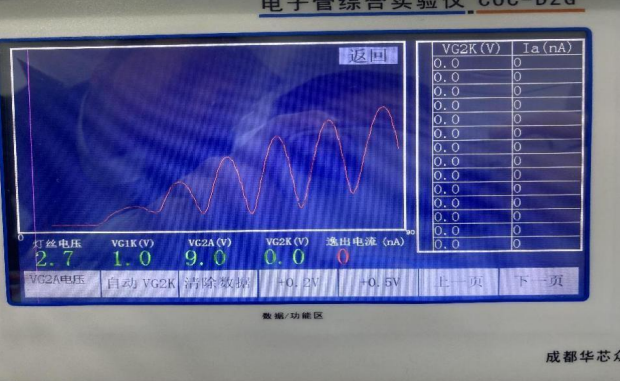
\includegraphics[clip,scale=0.05,trim={0 400 0 400}]{fig/fig12.jpg}
          				\caption{Lens measurement No. 3}
          				\label{figure.12}
          			\end{minipage}
          		\end{figure}
          		
    \begin{itemize}
    \item Measuring the focal length of a convex lens by primary imaging:\\
    On the precision guide, place the illuminator, the object screen (pintle screen or one-character screen or one-character needle), the convex lens to be measured and the image screen in turn, and adjust to the co-axis. Adjust the position of the convex lens or the object or image screen back and forth along the guide until a clear image is obtained on the image screen, note down the coordinates of the position of the object screen, convex lens and image screen, obtain the object and image distances and bring them into the formula to calculate the focal length f.
    \end{itemize}
     \begin{figure}[H]
            	     	\centering
            	     	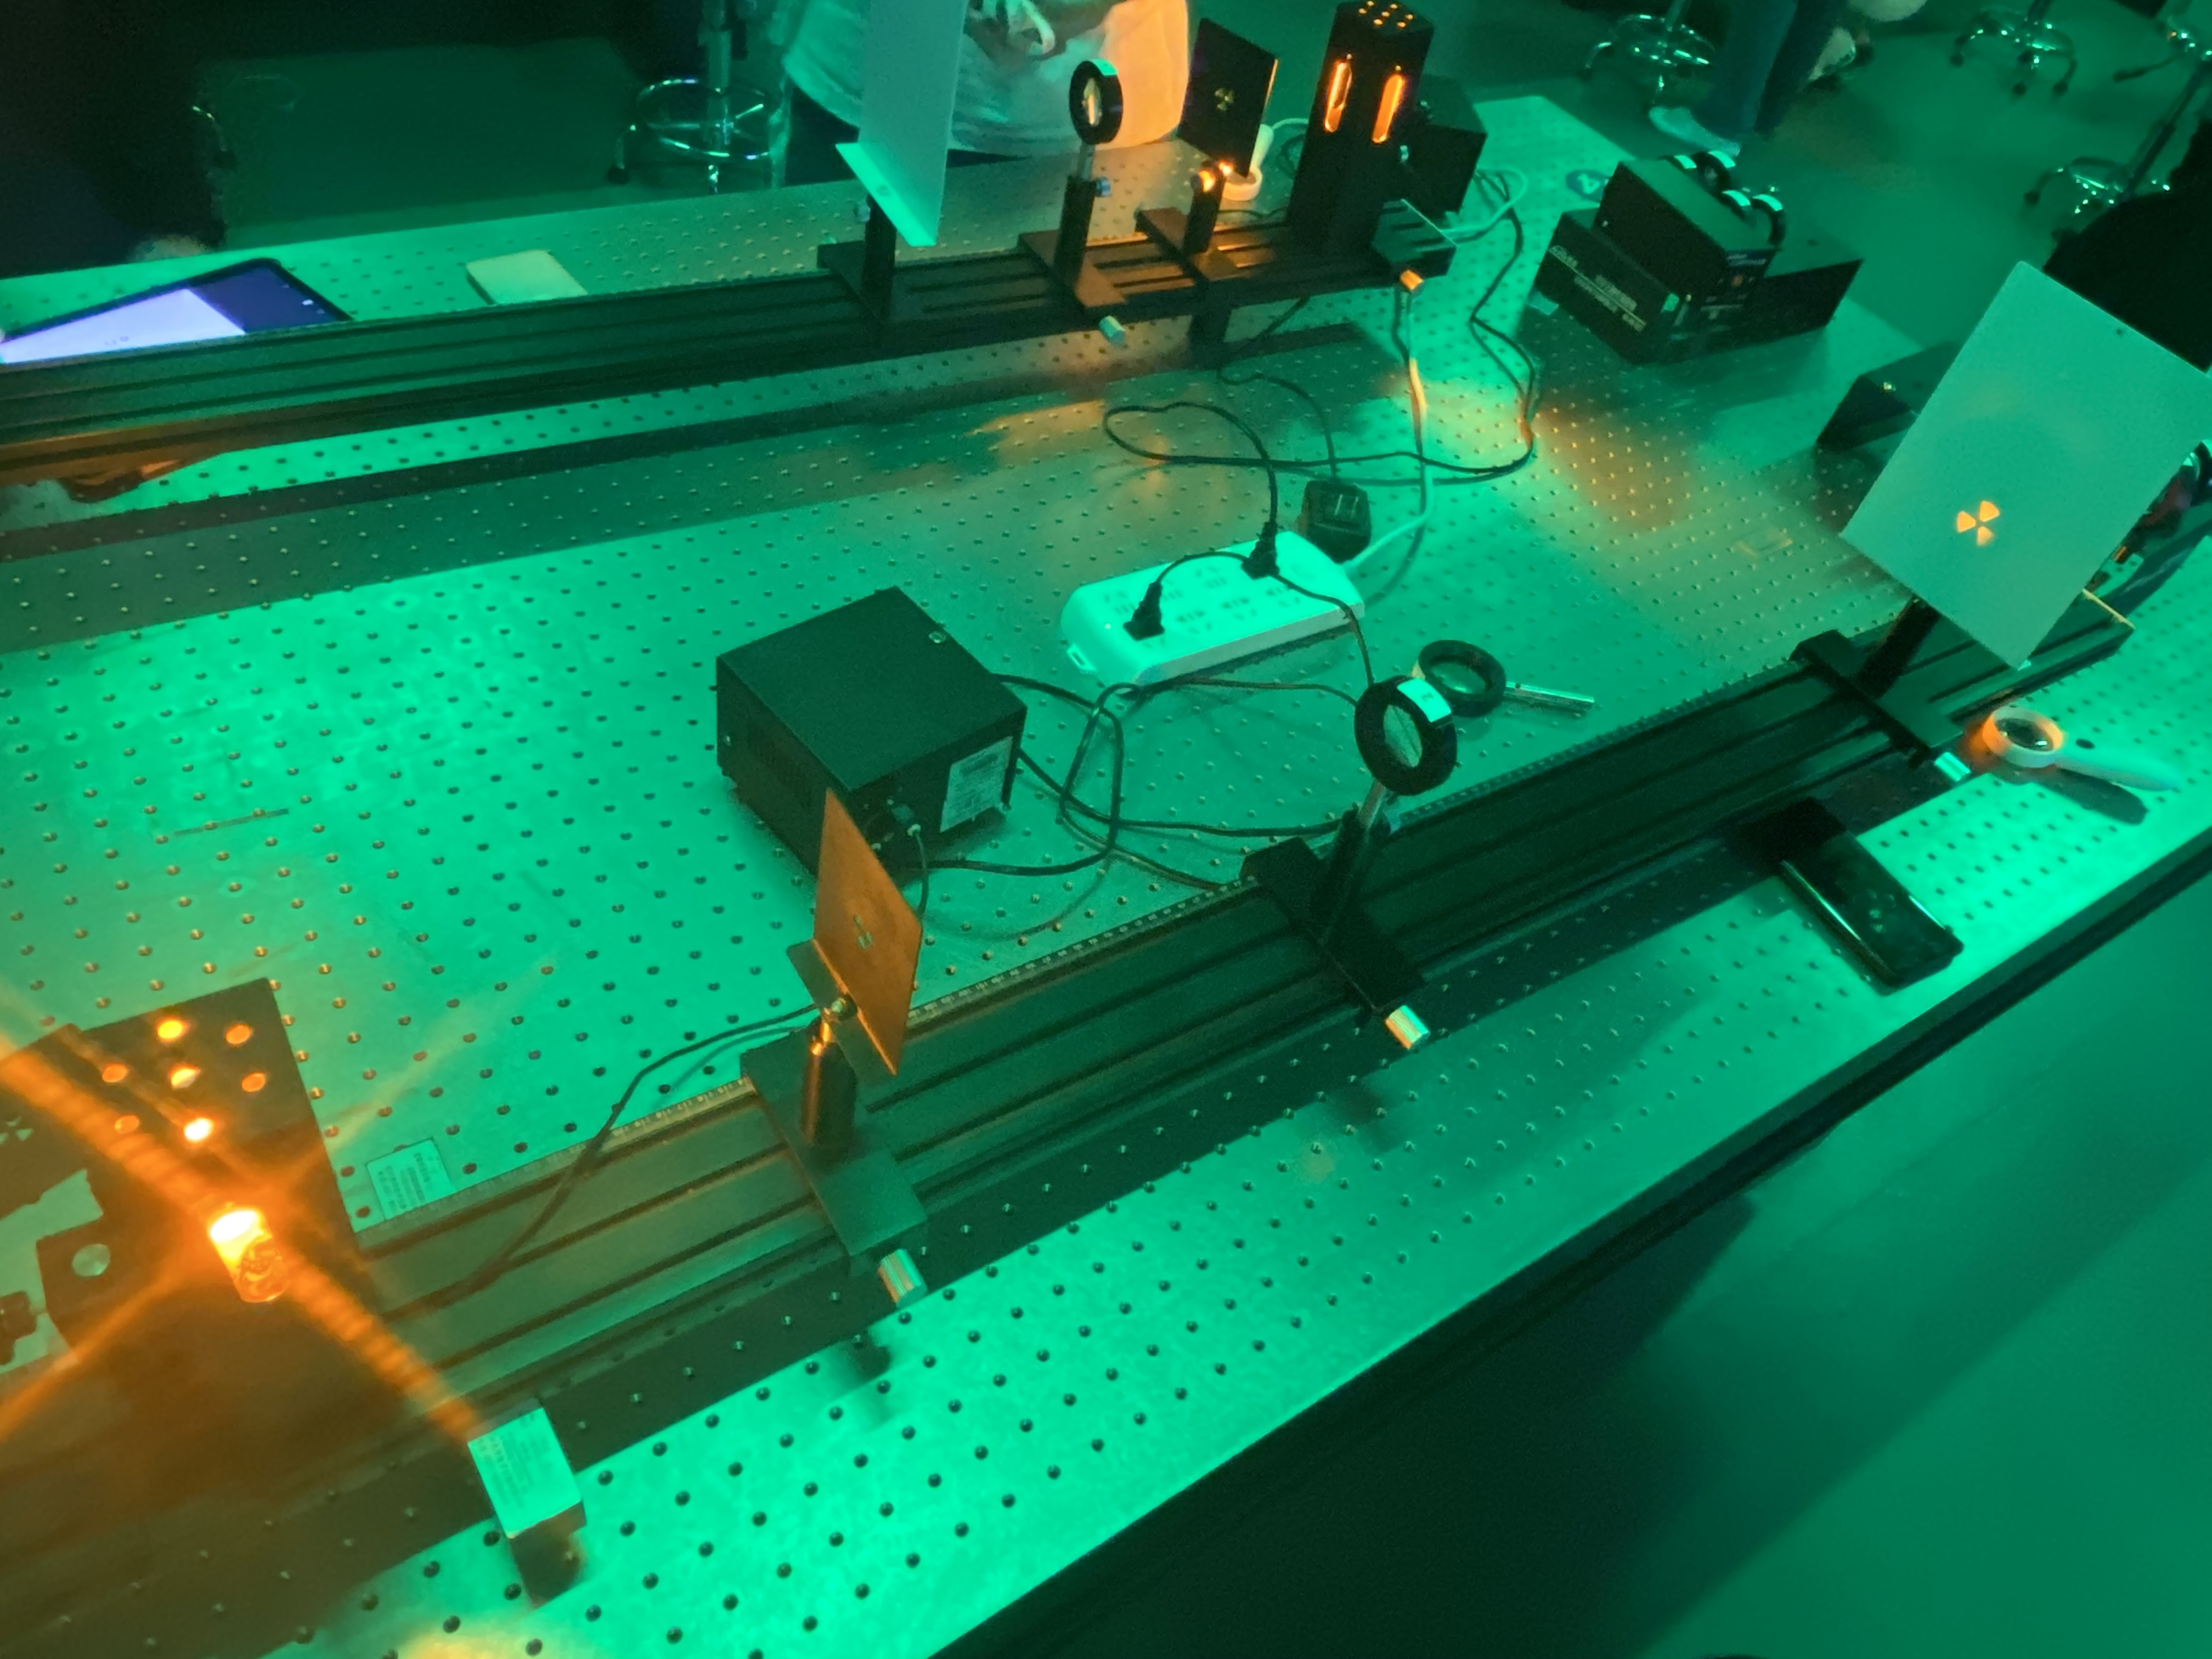
\includegraphics[clip,scale=0.07,trim={0 400 0 600}]{fig/fig13.jpg}
            	     	\caption{Co-axial adjustment}
            	     	\label{figure.13}
         \end{figure}
         
     \begin{itemize}
         \item Secondary imaging method for measuring the focal length of a convex lens:\\
         Choose different values of $D$ for $D > 4f$, move the lens $L$ so that the image screen appears as a clear magnified image and a reduced image respectively, record the coordinates of the object screen, the image screen and the positions of the magnified and reduced images, obtain the values of D and $d$ and substitute them into the formula to calculate the focal length.
     \end{itemize}
   
   \subsection{Measuring the focal length of a concave lens}
   The optical components are placed in accordance with the schematic optical path and the measurement procedure is as follows:
   \begin{itemize}
   \item Move the lens $L_1$ to form a reduced image $A'B'$ of object $AB$ on the screen, and record the position coordinate $x_1$ of the screen.
   \item Keeping the object and $L_1$ fixed, insert a concave lens $L_2$ between $L_1$ and the screen and adjust the position of the screen (or both $L_2$ and the screen, but $L_2$ cannot be moved beyond the original position of the screen) until a clear image of object $AB$ appears on the screen (preferably a reduced image). Record the position coordinates $x_2$ of $L_2$ and $x_3$ of the screen.
   \item Calculate the corresponding object distance $u$ and image distance $v$ based on the recorded values of $x_1$, $x_2$, and $x_3$:
   \end{itemize}
    \begin{eqnarray}
    u  =  -\left | x_1-x_2 \right | \qquad \upsilon  =  \left | x_3-x_2 \right |  
    \end{eqnarray}
    \begin{figure}[H]
                	     	\centering
                	     	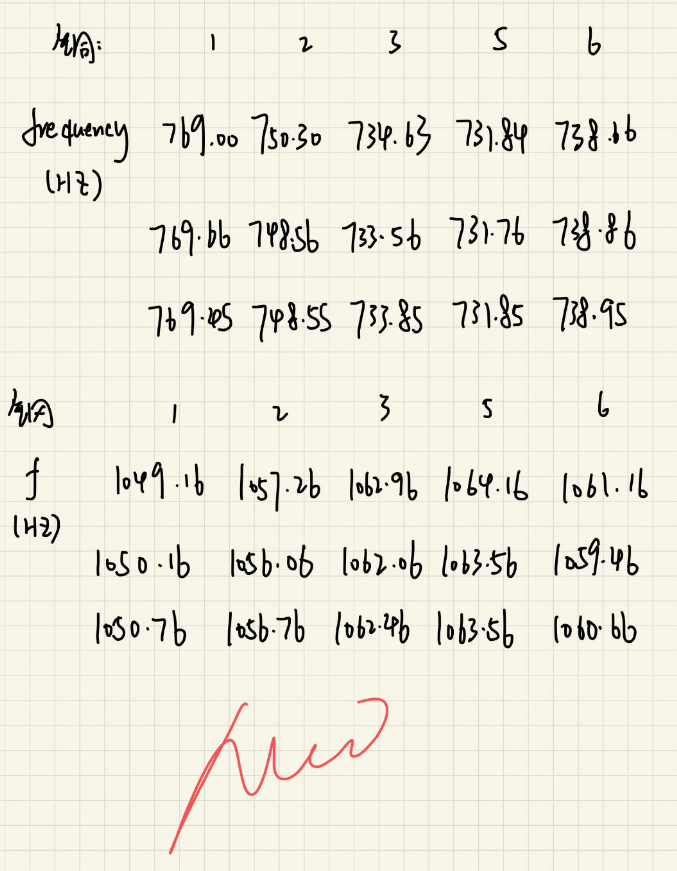
\includegraphics[clip,scale=0.07,trim={0 400 0 900}]{fig/fig14.jpg}
                	     	\caption{Object and image distance method for measuring the focal length of a concave lens}
                	     	\label{figure.14}
             \end{figure}
    
    
	
	\section{Data processing}
	The experiments were carried out as described above and the following data were subsequently obtained. An error analysis was done on the data and the corresponding results were obtained:
	\subsection{Measuring the focal length of a convex lens}
	\subsubsection{Parallel light focusing method}
   We followed the experimental procedure and measured the focal lengths of convex lens 2 and convex lens 3 using the parallel light method and calculated the average values recorded in the following table:
   
    	\begin{table}[H]
    	  \centering
    	  \caption{Parallel light measurement of focal length results}
    	    \begin{tabular}{ccc}
    	    \toprule[2pt]
    	    Number of measurements & Convex lens No. 2 & Convex lens No. 3 \\
    	    \midrule
    	    First time & 19.57cm & 25.75cm \\
    	    Second time & 19.48cm & 25.91cm \\
    	    Third time & 19.61cm & 25.83cm \\
    	    Mean value & 19.53cm & 25.83cm \\
    	    \bottomrule[2pt]
    	    \end{tabular}%
    	  \label{tab:addlabel}%
    	\end{table}%
    
    First we calculate the mean and standard deviation of the focal length of the convex lens 2 using the following formula,Here is an example of a convex lens 2:
    \begin{eqnarray}
    \overline{f}  =  \frac{\sum_{i  =  1}^{3} f_i}{3}  =  \frac{19.57+19.48+19.61}{3}  =  19.53cm
    \end{eqnarray}
    \begin{eqnarray}
    \sigma_f = \sqrt{\frac{ \sum_{i=1}^{3}(\overline{f}-f_i )^2}{3} } = 0.059cm
    \end{eqnarray}
    So as a result of the above equation we can conclude that the focal length of convex lens 2 is approximately:
    \begin{eqnarray}
    f_2 = 19.53 \pm 0.06cm
    \end{eqnarray}
    In the same way we can derive the focal length of convex lens 3:
    \begin{eqnarray}
        f_3 = 25.83 \pm 0.07cm
   \end{eqnarray}
    

    \subsubsection{Primary imaging method}
    Next we tried to measure the focal lengths of convex lenses 2 and 3 using the primary imaging method. We recorded $u$ and $v$ for each image and repeated the experiment three times in the following table:
    
    \begin{table}[H]
      \centering
      \caption{Results of focal length measurement by primary imaging}
        \begin{tabular}{ccccc}
        \toprule[2pt]
              & Measured values & \multicolumn{1}{l}{First time} &
              \multicolumn{1}{l}{Second time} & \multicolumn{1}{l}{Third time} \\
              \midrule
        \multirow{3}[4]{*}{Convex lens No. 2} & Object distance $u$(cm) & 31.5  & 26.52 & 30.41 \\
         \cmidrule{2-5}     & Image distance $v$(cm) & 51.31 & 72.51 & 54.21 \\
          \cmidrule{2-5}    & Focal length $f$(cm) & 19.51775148 & 19.41800666 & 19.48151855 \\
          \midrule
        \multirow{3}[4]{*}{Convex lens No. 3} & Object distance $u$(cm) & 39.6  & 42.31 & 46.42 \\
         \cmidrule{2-5}     & Image distance $v$(cm) & 73.52 & 65.89 & 56.73 \\
         \cmidrule{2-5}     & Focal length $f$(cm) & 25.73719943 & 25.76530407 & 25.52987494 \\
         \bottomrule[2pt]
        \end{tabular}%
      \label{tab:addlabel}%
    \end{table}%
    
    Where the focal length is calculated by the following formula:
    \begin{eqnarray}
        \frac{1}{\upsilon } +\frac{1}{u}  =  \frac{1}{f}  
        \end{eqnarray}
        
    Similarly to the error analysis process carried out when processing data on the focal length of convex lenses measured by parallel light, we also calculated the mean and standard deviation of the results obtained from focal length measurements using the primary imaging method, with the following results:
    \begin{align*}
     \overline{f_2}  =  19.47cm \qquad \qquad \sigma _2  = 0.0412cm\\
     \overline{f_3}  =  25.68cm \qquad \qquad \sigma _3  = 0.1050cm
    \end{align*}
    We can therefore obtain the focal length values obtained by this method
    \begin{align*}
    f_2 = 19.47\pm 0.05cm\\
    f_3 = 25.68  \pm 0.11cm
    \end{align*}
    
    \subsubsection{Secondary imaging method}
    Next we use the secondary imaging method to measure the focal lengths of convex lenses 2 and 3. Based on the experimental manipulations, we recorded the distance $d$ per movement of the convex lens and the distance $D$ from the object to the light screen, and recorded them in the following table:
    
    
  \begin{table}[htbp]
    \centering
    \caption{Results of the secondary imaging method for measuring the focal length of convex lenses}
      \begin{tabular}{ccccc}
       \toprule[2pt]
            & Measured values & \multicolumn{1}{l}{First time} & \multicolumn{1}{l}{Second time} & \multicolumn{1}{l}{Third time} \\
            \midrule
      \multirow{3}[4]{*}{Convex lens No. 2} & D (cm) & 81.29 & 86.27 & 99.15 \\
      \cmidrule{2-5}      & d (cm) & 17.58 & 27.18 & 45.73 \\
       \cmidrule{2-5}     & Focal length f (cm) & 19.37202516 & 19.42668512 & 19.51459808 \\
            \midrule
     \multirow{3}[4]{*}{Convex lens No. 3} & D (cm) & 117.42 & 105.5 & 110.87 \\
      \cmidrule{2-5}      & d (cm) & 41.32 & 18.31 & 30.67 \\
      \cmidrule{2-5}      & Focal length f (cm) & 25.71988162 & 25.58055427 & 25.59643727 \\
      \bottomrule[2pt]
      \end{tabular}%
    \label{tab:addlabel}%
  \end{table}%
  
    Where the focal length is calculated by the following formula:
    \begin{eqnarray}
    	f  =  \frac{D^2-d^2}{4D}  =  \frac{(D+d)(D-d)}{4D}  
    	\end{eqnarray}
        
    Similarly to the error analysis process carried out when processing data on the focal length of convex lenses measured by parallel light, we also calculated the mean and standard deviation of the results obtained from focal length measurements using the primary imaging method, with the following results:
    \begin{align*}
     \overline{f_2}  =  19.44cm \qquad \qquad \sigma _2  = 0.0588cm\\
     \overline{f_3}  =  25.63cm \qquad \qquad \sigma _3  = 0.0623cm
    \end{align*}
    We can therefore obtain the focal length values obtained by this method
    \begin{align*}
    f_2 = 19.44\pm 0.06cm\\
    f_3 = 25.63  \pm 0.07cm
    \end{align*}
    
    \subsection{General analysis of convex lens focal length data}
    Combining the first three methods of measuring the focal length of a convex lens, we obtain the following summary table of focal length measurements of convex lenses 2 and 3:
    \begin{table}[H]
          \centering
          \caption{Add caption}
            \begin{tabular}{cccc}
            \toprule[2pt]
                  & Focal length $f$(cm) & \multicolumn{1}{l}{Convex lens No. 2} & \multicolumn{1}{l}{Convex lens No. 3} \\
                  \midrule
             \multirow{3}[4]{*}{Parallel light focusing method} & First time & 19.57 & 25.75 \\
             \cmidrule{2-4}     & Second time & 19.48 & 25.91 \\
             \cmidrule{2-4}     & Third time & 19.61 & 25.83 \\
                  \midrule
             \multirow{3}[4]{*}{Primary imaging method} & First time & 19.52 & 25.74 \\
             \cmidrule{2-4}     & Second time & 19.42 & 25.77 \\
              \cmidrule{2-4}    & Third time & 19.48 & 25.53 \\
                  \midrule
            \multirow{3}[4]{*}{Secondary imaging method} & First time & 19.37 & 25.72 \\
              \cmidrule{2-4}    & Second time & 19.43 & 25.58 \\
             \cmidrule{2-4}     & Third time & 19.51 & 25.59 \\
                   \bottomrule[2pt]
            \end{tabular}%
          \label{tab:addlabel}%
        \end{table}%
        
        For the information in the table, we tried to remove outliers. Two methods were used to identify outliers: one was to analyse the data for outliers by plotting a standard box plot, and the other was to calculate the mean and standard deviation, treating data that were more or less than double the standard deviation of the mean as outliers (marked as red dots in the graph). Box line plots and scatter plots based on the above approaches are as follows:
        
        Analysis of focal length data for convex lens No. 2:
        \begin{figure}[H]
                  			\begin{minipage}[t]{0.5\linewidth}
                  				\centering
                  				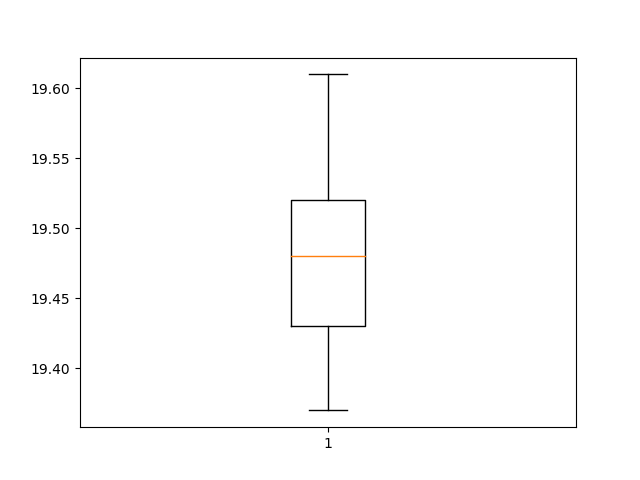
\includegraphics[clip,scale=0.45,trim={0 0 0 0}]{fig/fig15.png}
                  				\caption{Box line chart outlier analysis}
                  				\label{figure.15}
                  			\end{minipage}
                  			\begin{minipage}[t]{0.5\linewidth}
                  				\centering
                  				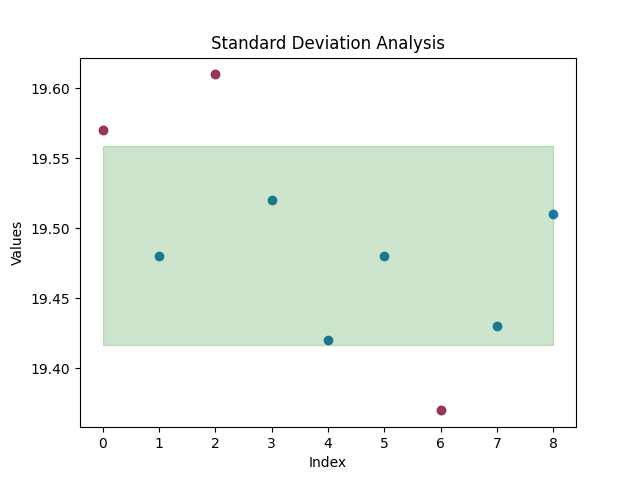
\includegraphics[clip,scale=0.45,trim={0 0 0 0}]{fig/fig16.png}
                  				\caption{Scatter plot outlier analysis}
                  				\label{figure.16}
                  			\end{minipage}
                  		\end{figure}
                  		
        Analysis of focal length data for convex lens No. 3:
        \begin{figure}[H]
                          			\begin{minipage}[t]{0.5\linewidth}
                          				\centering
                          				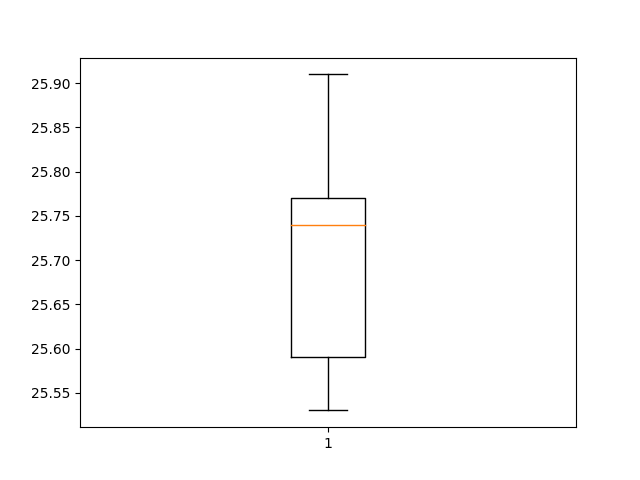
\includegraphics[clip,scale=0.45,trim={0 0 0 0}]{fig/fig17.png}
                          				\caption{Box line chart outlier analysis}
                          				\label{figure.17}
                          			\end{minipage}
                          			\begin{minipage}[t]{0.5\linewidth}
                          				\centering
                          				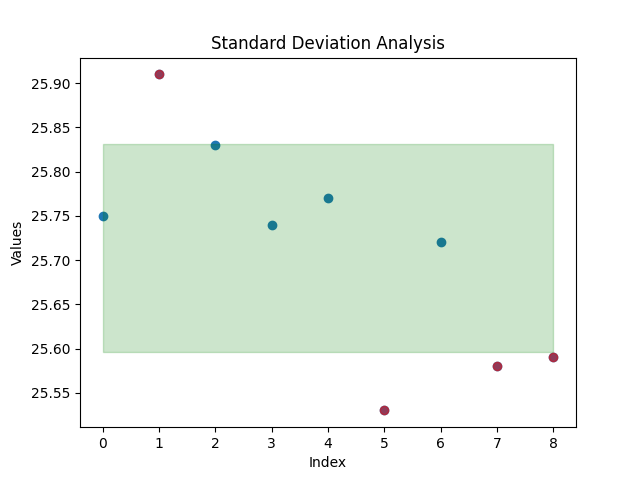
\includegraphics[clip,scale=0.45,trim={0 0 0 0}]{fig/fig18.png}
                          				\caption{Scatter plot outlier analysis}
                          				\label{figure.18}
                          			\end{minipage}
                          		\end{figure}
                          		
        From the graph, we can see that there are no obvious outliers for $f_1$ and $f_2$ when using the box line plot, whereas there are outliers for $f_1$ and $f_2$ in the three-point plot. The reason for this is probably because the data volume is too small to use a box line plot to analyse the data structure in a suitable way, so we use a scatter plot to find the outliers.
        
        After eliminating the outliers, we recalculated the focal lengths of the two lenses as follows:
        \begin{align*}
             \overline{f_2}  =  19.47cm \qquad \qquad \sigma _2  = 0.0373cm\\
             \overline{f_3}  =  25.76cm \qquad \qquad \sigma _3  = 0.0376cm
            \end{align*}
            We can therefore obtain the focal length values obtained by this method
            \begin{align*}
            f_2 = 19.47\pm 0.04cm\\
            f_3 = 25.76  \pm 0.04cm
            \end{align*}
        



    \subsection{Measuring the focal length of a concave lens}
    Next we will measure the focal length of a concave lens using the object-image distance method. Based on the principle of the experiment and the specific procedure, we measured and recorded the object distance $u$ and image distance $v$ and filled in the following table:
    \begin{table}[H]
      \centering
      \caption{Results of measuring the focal length of a concave lens}
        \begin{tabular}{cccc}
        \toprule[2pt]
        Concave lens No. 4 & \multicolumn{1}{l}{First time} & \multicolumn{1}{l}{Second time} & \multicolumn{1}{l}{Third time} \\
         \midrule
        Object distance \$u\$(cm) & 4.01  & 4.56  & 4.47 \\
        Image distance \$v\$(cm) & 11.72 & 24.1  & 19.01 \\
        Focal length \$f\$(cm) & 6.095616083 & 5.624155578 & 5.844202201 \\
         \bottomrule[2pt]
        \end{tabular}%
      \label{tab:addlabel}%
    \end{table}%
    Where the focal length is calculated by the following formula:
       \begin{eqnarray}
           \frac{1}{f}  = \frac{1}{u}-\frac{1}{\upsilon }   
           \end{eqnarray}
           
            
        Similarly to the error analysis process carried out when processing data on the focal length of convex lenses measured by parallel light, we also calculated the mean and standard deviation of the results obtained from focal length measurements using the primary imaging method, with the following results:
        \begin{align*}
         \overline{f_4}  =  5.85cm \qquad \qquad \sigma _4  = 0.1926cm
        \end{align*}
        We can therefore obtain the focal length values obtained by this method
        \begin{align*}
        f_4 = 5.85\pm 0.19cm
        \end{align*}
    
    
    
\section{Conclusion and analysis}
\subsection{Experimental conclusion}

Based on the information from the data obtained from the experiments and the results of the data processing, we can obtain the focal lengths of the three lenses measured:

\begin{align*}
f_2 = 19.47\pm 0.04cm\\
f_3 = 25.76  \pm 0.04cm\\
f_4 = 5.85\pm 0.19cm
\end{align*}

The above data allows for the basic determination of the focal lengths of the three lenses, but there is a certain amount of random error and systematic error in the measurement process. The focal length of the convex lens was measured in three different ways, and the data was processed and analysed as a whole, so the focal length of the convex lens was measured more accurately. The focal length measurement of the concave lens is less accurate due to the large systematic error and the small number of experimental methods and samples used. The specific error analysis will be explained later.

\subsection{Experimental error analysis}
\begin{itemize}
\item Parallel light method for measuring convex lens focal length:
\begin{itemize}
\item Random error: Mainly caused by errors in measuring the distance of parallel light, which may be due to uneven placement or non-straight light, etc.
\item Systematic error: Possible due to zero error of measuring instruments, non-ideal nature of the instrument, etc.
\end{itemize}
\item One-point imaging method for measuring convex lens focal length:
\begin{itemize}
\item Random error: Mainly caused by errors in imaging position, which may be due to improper observation angle or inaccurate imaging position, etc.
\item Systematic error: Possible due to inaccurate position of lens and ruler, imaging distance error, etc.
\end{itemize}
\item Two-point imaging method for measuring convex lens focal length:
\begin{itemize}
\item Random error: Mainly caused by errors in imaging position and measuring length, which may be due to improper human operation or low precision of measuring instruments, etc.
\item Systematic error: Possible due to inaccurate position of lens and ruler, light source position error, etc.
\end{itemize}
\item Object distance-image distance method for measuring concave lens focal length:
\begin{itemize}
\item Random error: Mainly caused by errors in imaging position, which may be due to improper observation angle or inaccurate imaging position, etc.
\item Systematic error: Possible due to inaccurate position of lens and ruler, imaging distance error, etc.
\end{itemize}
\end{itemize}

\begin{appendix}
	\section{Documentation of experimental procedures}
\begin{figure}[H]
                          			\begin{minipage}[t]{0.5\linewidth}
                          				\centering
                          				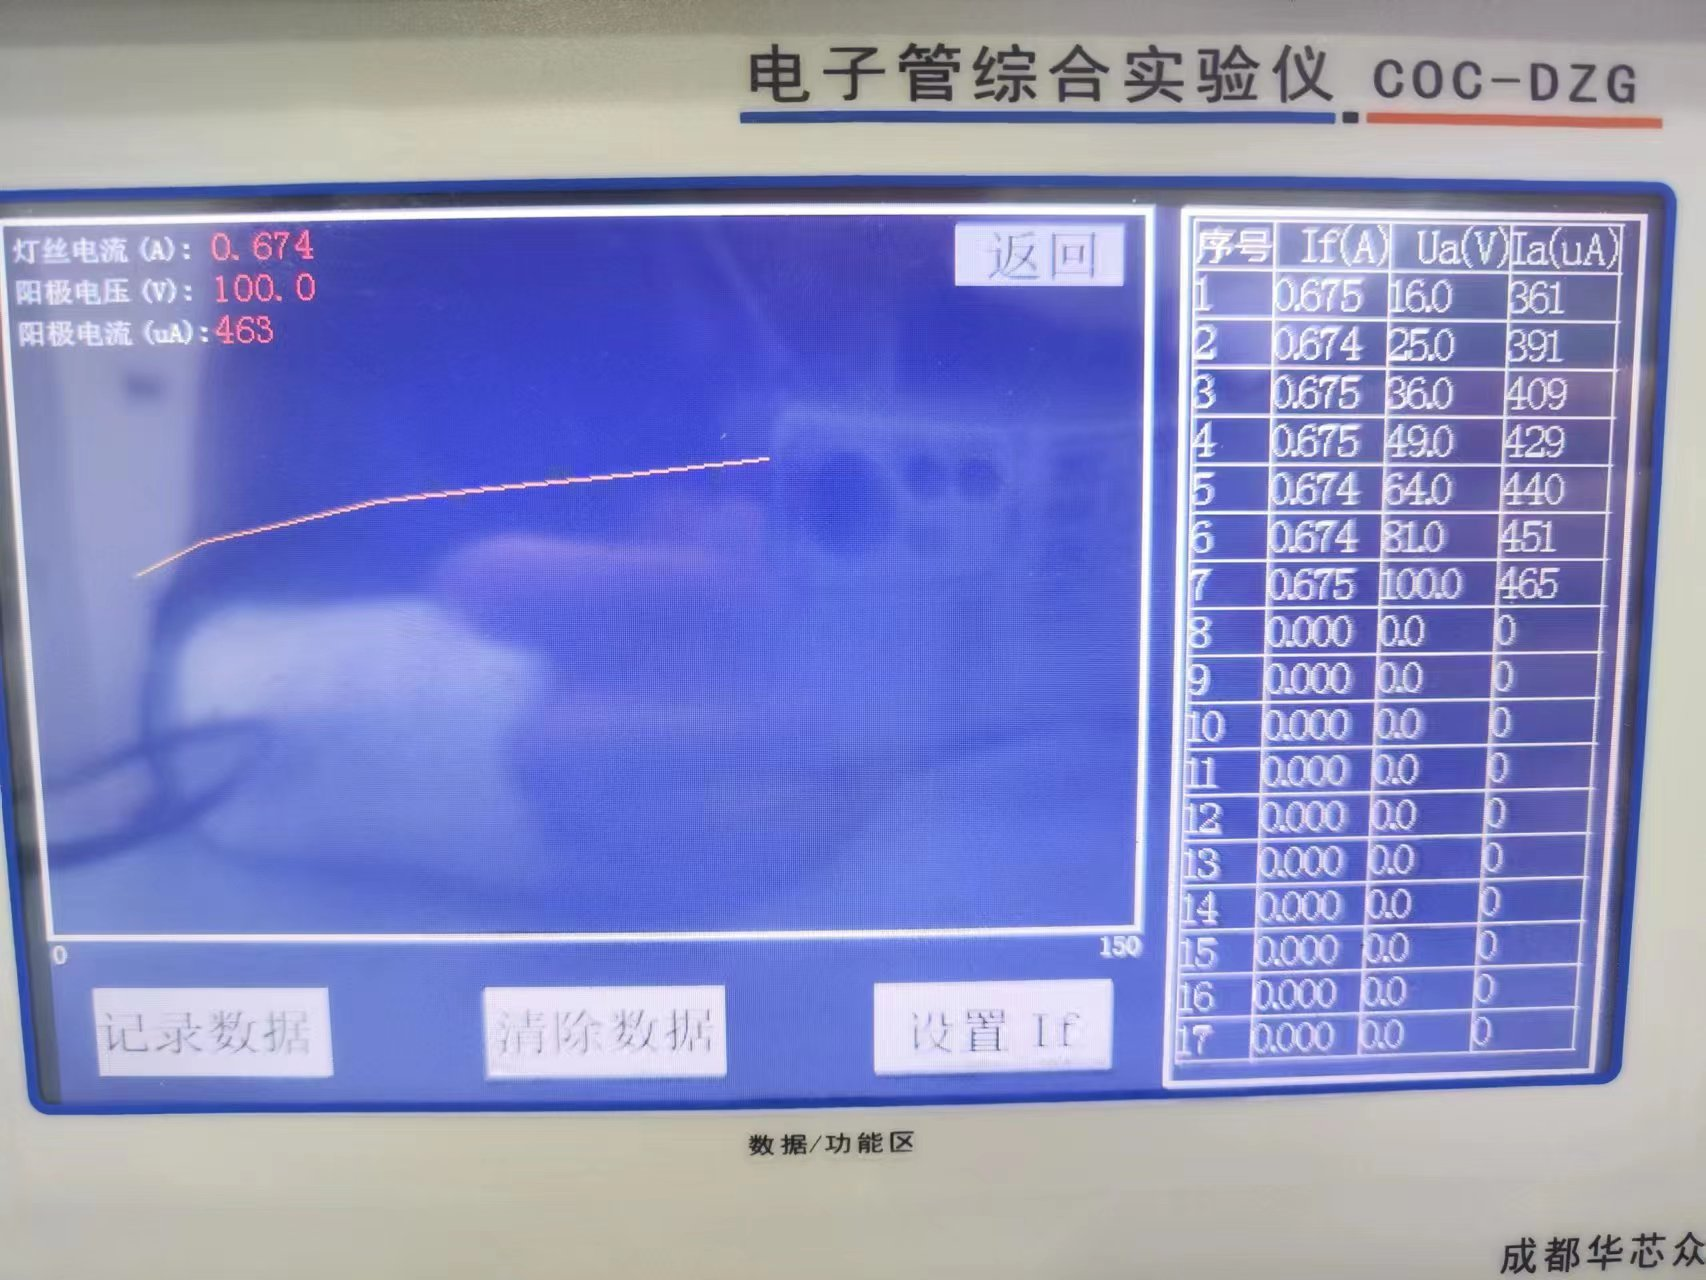
\includegraphics[clip,scale=0.05,trim={0 0 0 0}]{fig/fig19.jpg}
                          			
                          				\label{figure.19}
                          			\end{minipage}
                          			\begin{minipage}[t]{0.5\linewidth}
                          				\centering
                          				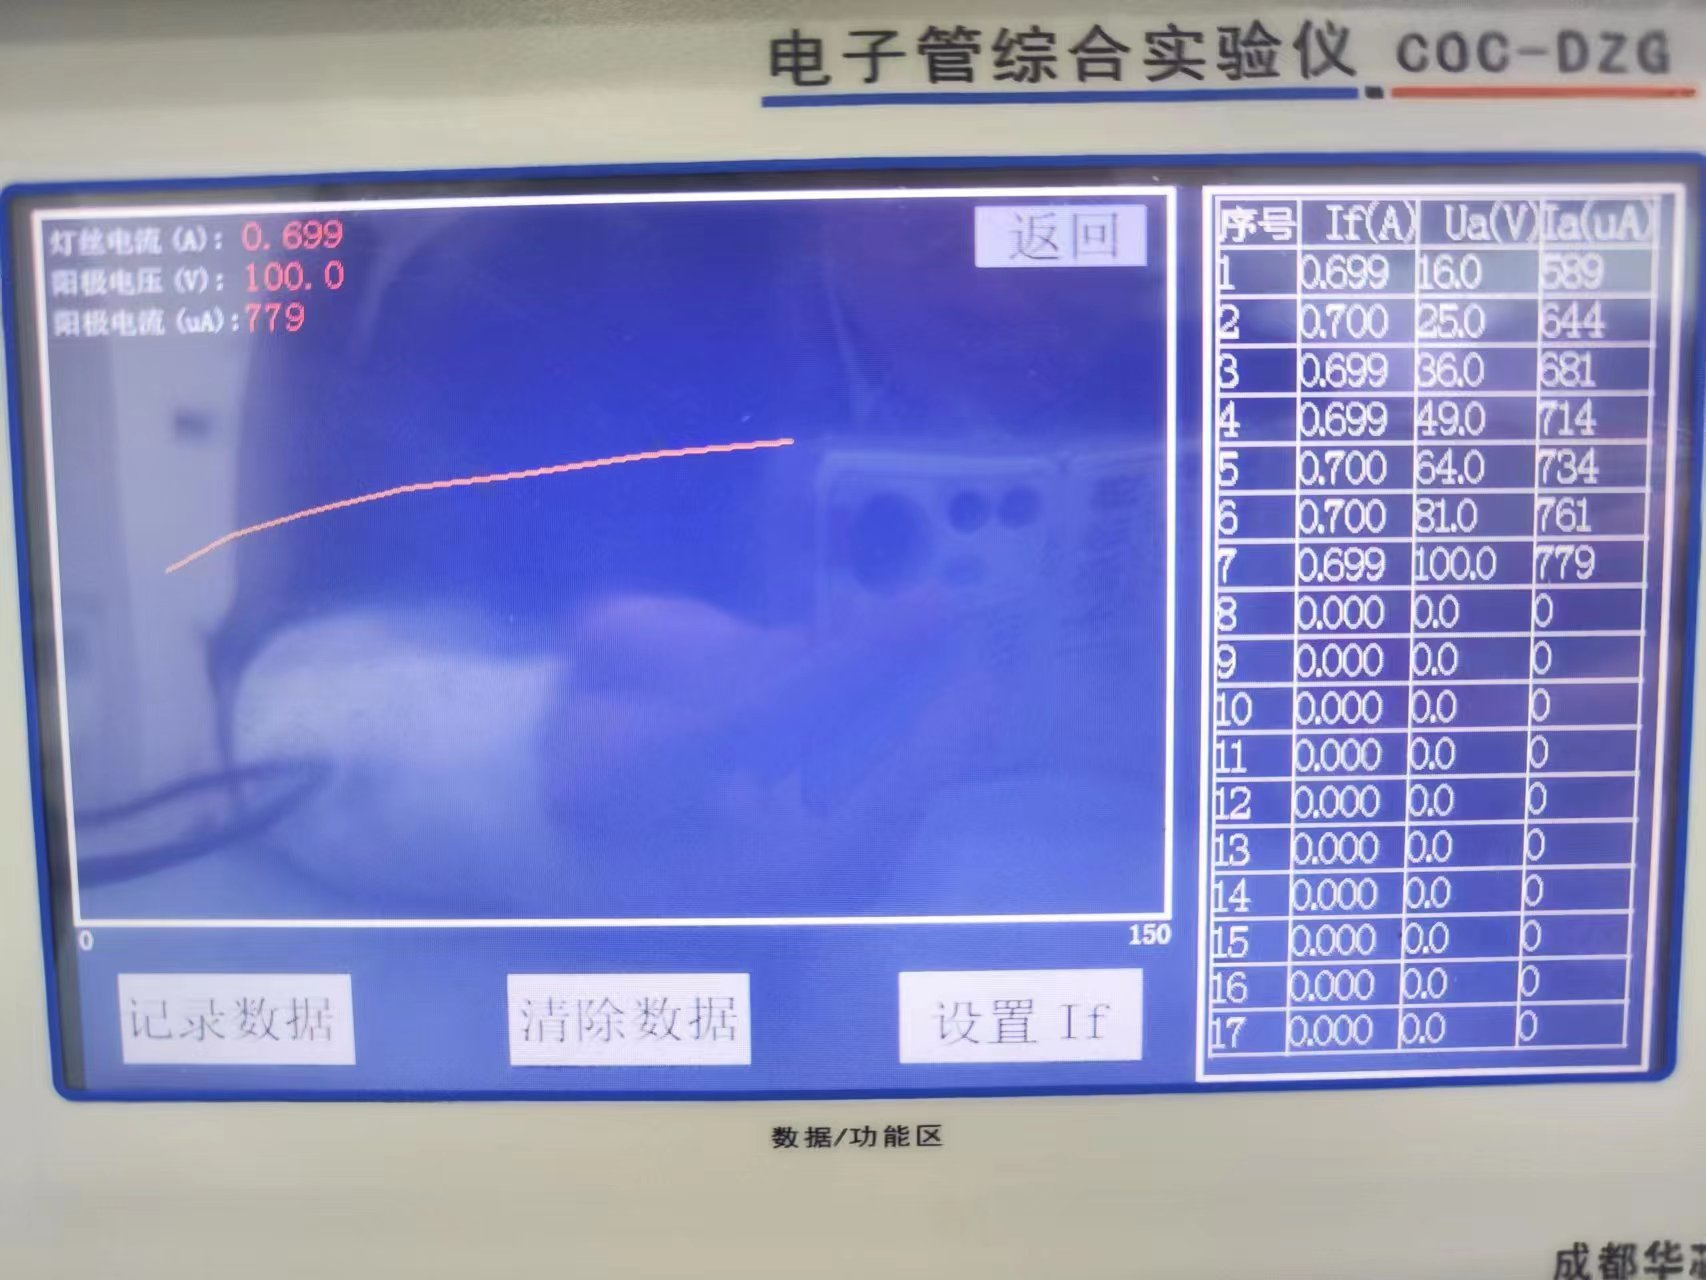
\includegraphics[clip,scale=0.05,trim={0 0 0 0}]{fig/fig20.jpg}
                          				
                          				\label{figure.20}
                          			\end{minipage}
                          		\end{figure}
	
	\section{Data Analysis and Visualisation Source Code}
	\subsection{Calculation of data means and standard deviations}
	\begin{lstlisting}[language=python]
import numpy as np
import matplotlib.pyplot as plt
# 定义数据
data = [25.75,  25.83, 25.74, 25.77,  25.72]
mean = np.mean(data)
std = np.std(data)
print(mean,std)
	\end{lstlisting}
	
	\subsection{Box line charting and outlier analysis}
	\begin{lstlisting}[language=python]
import numpy as np
import matplotlib.pyplot as plt

# 读取数据
#data = np.array([19.57, 19.48, 19.61, 19.52, 19.42, 19.48, 19.37, 19.43, 19.51])
data = np.array([25.75, 25.91, 25.83, 25.74, 25.77, 25.53, 25.72, 25.58, 25.59])

# 绘制箱线图
fig, ax = plt.subplots()
ax.boxplot(data)

# 标记异常值
q1 = np.percentile(data, 25)
q3 = np.percentile(data, 75)
iqr = q3 - q1
upper_bound = q3 + 1.5 * iqr
lower_bound = q1 - 1.5 * iqr
outliers = [x for x in data if x < lower_bound or x > upper_bound]
ax.plot(np.ones(len(outliers)), outliers, 'ro', alpha=0.5)

# 显示图形
plt.show()
		\end{lstlisting}
		
	\subsection{Scatter plot production and outlier analysis}
		\begin{lstlisting}[language=python]
import numpy as np
import matplotlib.pyplot as plt

# 读取数据
#data = np.array([19.57, 19.48, 19.61, 19.52, 19.42, 19.48, 19.37, 19.43, 19.51])
data = np.array([25.75, 25.91, 25.83, 25.74, 25.77, 25.53, 25.72, 25.58, 25.59])

# 计算平均值和标准差
mean = np.mean(data)
std = np.std(data)

# 计算异常值阈值
threshold = mean +  std
down = mean -  std
# 绘制散点图
fig, ax = plt.subplots()
ax.scatter(range(len(data)), data)

# 标记异常值
outliers = [x for x in data if x > threshold or x<down]
ax.plot([i for i in range(len(data)) if data[i] in outliers], outliers, 'ro', alpha=0.5)

# 添加阴影
x = np.linspace(0, len(data)-1, 100)
y1 = mean - std
y2 = mean + std
ax.fill_between(x, y1, y2, alpha=0.2, color='green')

# 设置图形属性
ax.set_title('Standard Deviation Analysis')
ax.set_xlabel('Index')
ax.set_ylabel('Values')

# 显示图形
plt.show()

		\end{lstlisting}

\end{appendix}


\end{document}  